\documentclass[a4paper, 12pt]{article} % тип документа

%%%Библиотеки
	%\usepackage[warn]{mathtext}	
	\usepackage[T2A]{fontenc}   %Кодировка
	\usepackage[utf8]{inputenc} %Кодировка исходного текста
	\usepackage[english, russian]{babel} %Локализация и переносы
	\usepackage{caption}
	\usepackage{listings}
	\usepackage{amsmath, amsfonts, amssymb, amsthm, mathtools}
	\usepackage[warn]{mathtext}
	\usepackage[mathscr]{eucal}
	\usepackage{wasysym}
	\usepackage{graphicx} %Вставка картинок правильная
	\DeclareGraphicsExtensions{.pdf,.png,.jpg}
	\graphicspath{ {images/} }
	
	\setlength{\parskip}{0.5cm}
	
	\usepackage{pgfplots}
	\usepackage{indentfirst}
	\usepackage{float}    %Плавающие картинки
	\usepackage{wrapfig}  %Обтекание фигур (таблиц, картинок и прочего)
	\usepackage{fancyhdr} %Загрузим пакет
	\usepackage{lscape}
	\usepackage{xcolor}
	\usepackage[normalem]{ulem}
	\usepackage{wasysym}
	\usepackage{subfig}
	\usepackage{graphicx}
	
	\usepackage{titlesec}
	\titlelabel{\thetitle.\quad}

	\usepackage{hyperref}
	\newenvironment{comment}{}{}

%%%Конец библиотек

%%%Настройка ссылок
%%%	\hypersetup
%%%	{
%%%		colorlinks = true,
%%%		linkcolor  = blue,
%%%		filecolor  = magenta,
%%%		urlcolor   = blue
%%%	}
%%%Конец настройки ссылок


%%%Настройка колонтитулы
    \pagestyle{fancy}
    \fancyhead{}
    \fancyhead[L]{1.1.1}
    \fancyhead[R]{Засимов Георгий, группа Б01-109}
    \fancyfoot[C]{\thepage}
%%%конец настройки колонтитулы



\begin{document}

%%%Начало титульника
\begin{titlepage}

    \newpage
    \begin{center}
        \normalsize Московский физико-технический институт \\(национальный исследовательский университет)
    \end{center}

    \vspace{6em}

    \begin{center}
        \Large Лабораторная работа по общему курсу физики\\
    \end{center}

    \vspace{1em}

    \begin{center}
        \Large \textbf{Отчёт о выполнении лабораторной работы 1.3.1\\ {Определение модуля Юнга на основе исследования деформаций растяжения проволоки.}}
    \end{center}

    \vspace{2em}

    \begin{center}
        \large Засимов Георгий Алексеевич \\
        Группа Б01-109
    \end{center}

    \vspace{\fill}

    \begin{center}
    Долгопрудный \\2021
    \end{center}
    
\end{titlepage}
%%%Конец Титульника

\newpage

%\\\\\\\\\\\\\\\\\\\\\\\\\\\\\\\\\\\\\\\\\\\\\\\\\\\\\\\\\\\\\\\\\\\\\\\\\\\\
\section{Аннотация}


    В данной работе мы экспериментаьно получили зависимость между напряжением и деформацией (закон Гука) для одноостного растяжения. Сравнили с теоретическим описанием зависимости. Вычислили модуль Юнга по результатам измерений и определили по нему материал проволоки.
    
    
    
    
%----------------------------------------------------   
\section{Теоретические сведения и методика измерений}

    В работе исследуется растяжение проволоки, что соответствует одноостному напряженному состоянию, которое описывается формулой:
    
\begin{equation} \label{закон гука}
    \sigma = E \varepsilon
\end{equation}

    где $\sigma = \frac{F}{s} $ - напряжение, $\varepsilon = \frac{dl}{l}$ - деформация в точке, Е - модуль Юнга.\\
    
    Поскольку
    
\begin{equation} \label{закон гука 2}
    \sigma = \frac{F}{s} = \frac{k \Delta l}{s} => E = \frac{Fl}{s \Delta l}
\end{equation}

    То модуль Юнга вычисляется по формуле:
    
\begin{equation} \label{модуль}
    E = \frac{kl}{s}
\end{equation}

    где $k$ - коэффициент жесткости металла, который найдем в ходе эксперимента.




%-----------------------------------------------------
\section{Оборудование и экспериментальные погрешности}
%----------
\subsection{Экспериментальная установка и методика измерений}

    Для определения модуля Юнга используется прибор Лермантова, схема которого изображена на рис. 1.
    
\begin{center}
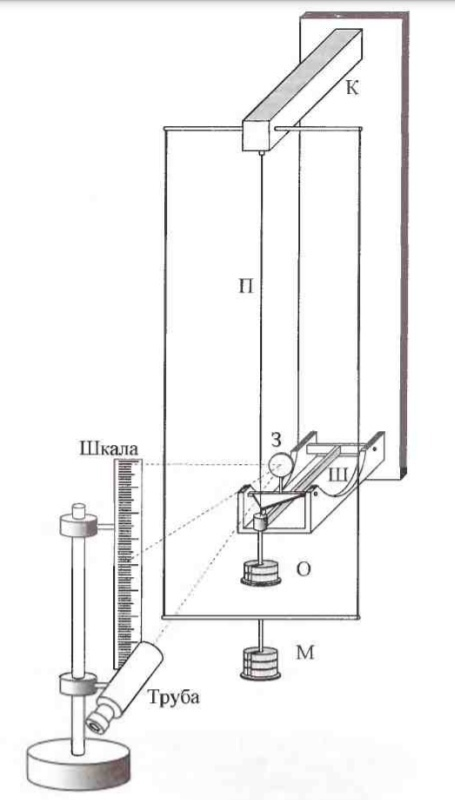
\includegraphics[width=5cm, height=10cm]{lermant.jpeg}
\end{center}

\begin{flushright}
{\scriptsize \textbf{Рис. 1} \textbf {Прибор Лермантова.}}
\end{flushright}

    (П - проволока, К - консоль, Ш - шарнирный  кронштейн, З - зеркало, М, О - площадки длял грузов, $r$ - рычаг).
    
    Натяжение проволки меняется при перекладывании грузов с площадки М на площадку О, при этом напряжение, действующее на кронштейн остается неизменным. Это позволяет исключить влияние деформации кронштейна на точность измерений. Отметим, что при малых нагрузках проволока распрямляется, а не растягивается, поэтому измерения при первых грузах не будут соответствоать искомой зависимости.
%----------
\subsection{Погрешности измерений}

    Определим диаметр проволоки, длину рычага $r$, длину проволоки и расстояние от шкалы до зеркала:\\
    
    примем значения диаметра проволоки и длины рычага с высокой точностью (поскольку это данные прибора, $\varepsilon_r = \varepsilon_l \approx 0 \%$):
    
\[r = 13 mm\]
\[d = 0,73 mm\]

    Тогда площадь поперечного сечения проволоки будет вычислена:
    
\[s = \frac{\pi d^4}{4} = 0,419 mm^2\]

    Длина проволоки и расстояние от зеркала до шкалы измерялись линейкой с $\sigma_l = 10 mm$:
    
\[l = 176,3 \pm 1,0 cm (\varepsilon = 0,6 \%)\]
\[h = 139,5 \pm 1,0 cm (\varepsilon = 0,7 \%)\]

    Также будем учитывать погрешность шкалы $\varepsilon = 0,05$ дел.\\


    Формула, описывающая зависимость удлинения проволоки $\Delta l$ от расстояния $h$, длины рычага $r$  и разности количества делений шкалы $\Delta n = n - n_0$, где $n_0$ - начальное значение по шкале, получается из закона гука \eqref{закон гука 2} и следующих уравнений:
    
    при удлинении проволоки на $\Delta l$ зеркало повернется на угол $\phi$, в то же время изменение положения зеркальца фиксируется на шкале, которую наблюдающий видит через трубу, тогда тангенс угла $\phi$ зависит и от изменения показаний шкалы $\Delta n$ и расстояния от зеркальца до шкалы $h$ (см. рис. 2). Поскольку $\Delta l$ и $\phi$ малы, имеем:
    
\[tg\phi = \frac{\Delta l}{r}\]
\[tg2\phi = \frac{\Delta n}{h} = 2 tg\phi => \Delta l = r tg\phi = \frac{r \Delta n}{2h}\]
    
\begin{equation} \label{dl}
    \Delta l = \frac{r \Delta n}{2h}
\end{equation}


\begin{center}
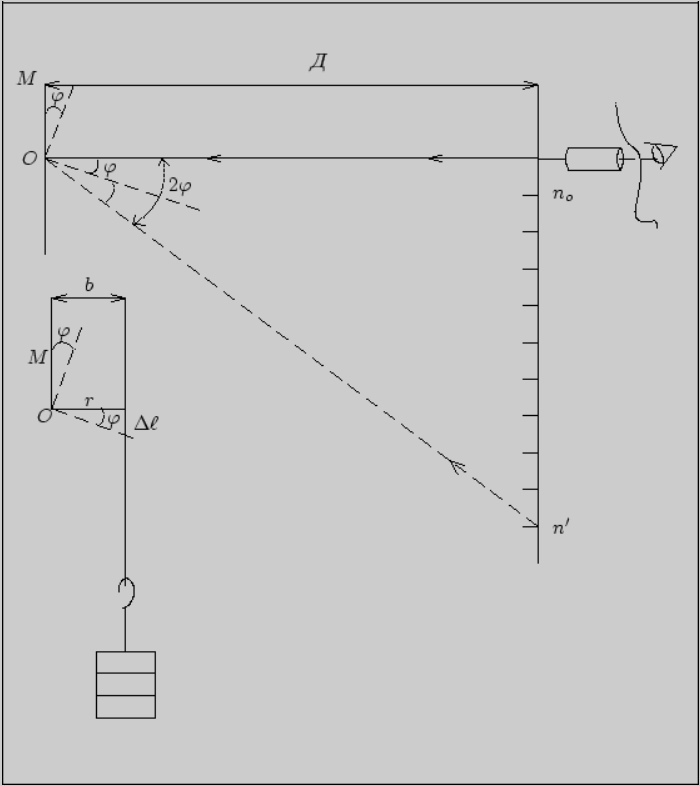
\includegraphics[width=7cm, height=8cm]{deltal.jpeg}
\end{center}
\begin{flushright}
{\scriptsize \textbf{Рис. 2.} \textbf {Удлинение проволоки и прибор Лермантова.}}
\end{flushright}


%------------------------------------------------
\section{Результаты измерений и обработка данных}

    Значения массы для каждого груза представлены в таблице 1. Полученные в ходе эксперимента данные представлены в таблице 2 для $I$, $II$ и $III$ серий измерений соответственно. Начальное значение $n_0 = 2,9$ при 1 грузе массой $= 245,8$ г.
    
    
\begin{table}[H]
\centering
\begin{tabular}{|l|l|}
\hline
№ груза & масса, г \\ \hline
1       & 245,8    \\ \hline
2       & 246,12   \\ \hline
3       & 245,7    \\ \hline
4       & 245      \\ \hline
5       & 246,1    \\ \hline
6       & 245,5    \\ \hline
7       & 245,6    \\ \hline
8       & 245,5    \\ \hline
9       & 245,6    \\ \hline
10      & 245,2    \\ \hline
\end{tabular}
\end{table}
 
\begin{flushright}
{\scriptsize \textbf{Таблица 1.} \textbf {Массы грузов.}}
\end{flushright}  
 

\newpage
\begin{table}[H]
\centering
\begin{tabular}{|l|l|l|l|}
\hline
серия     & I          & II         & III        \\ \hline
N, грузов & n, делений & n, делений & n, делений \\ \hline
1         & 2,9        & 3,2        & 3,3        \\ \hline
2         & 4,3        & 4,6        & 4,4        \\ \hline
3         & 5,5        & 6          & 5,5        \\ \hline
4         & 6,6        & 7,3        & 6,9        \\ \hline
5         & 7,8        & 8,3        & 7,9        \\ \hline
6         & 9,2        & 9,5        & 9,1        \\ \hline
7         & 10,6       & 10,7       & 10,3       \\ \hline
8         & 11,5       & 11,8       & 11,5       \\ \hline
9         & 12,6       & 12,9       & 12,2       \\ \hline
10        & 13,8       & 14         & 13,7       \\ \hline
9         & 12,8       & 12,9       & 12,6       \\ \hline
8         & 11,7       & 11,7       & 11,4       \\ \hline
7         & 10,5       & 10,2       & 10,2       \\ \hline
6         & 9,2        & 9          & 8,9        \\ \hline
5         & 8,1        & 7,7        & 7,7        \\ \hline
4         & 6,8        & 6,3        & 6,4        \\ \hline
3         & 5,7        & 5,1        & 5,2        \\ \hline
2         & 4,4        & 4,1        & 3,6        \\ \hline
1         & 3,2        & 3          & 2,8        \\ \hline
\end{tabular}
\end{table}  
    
\begin{flushright}
{\scriptsize \textbf{Таблица 2.} \textbf {Результаты измерений для 3 серий.}}
\end{flushright}    


    Построим график зависимости удлинения проволоки $\Delta l$ (см формулу \eqref{dl}) от нагрузки Р $= g*m$ (примем $g = 9,81$ м/$с^2$) (см Рис. 3). 
    
\begin{center}
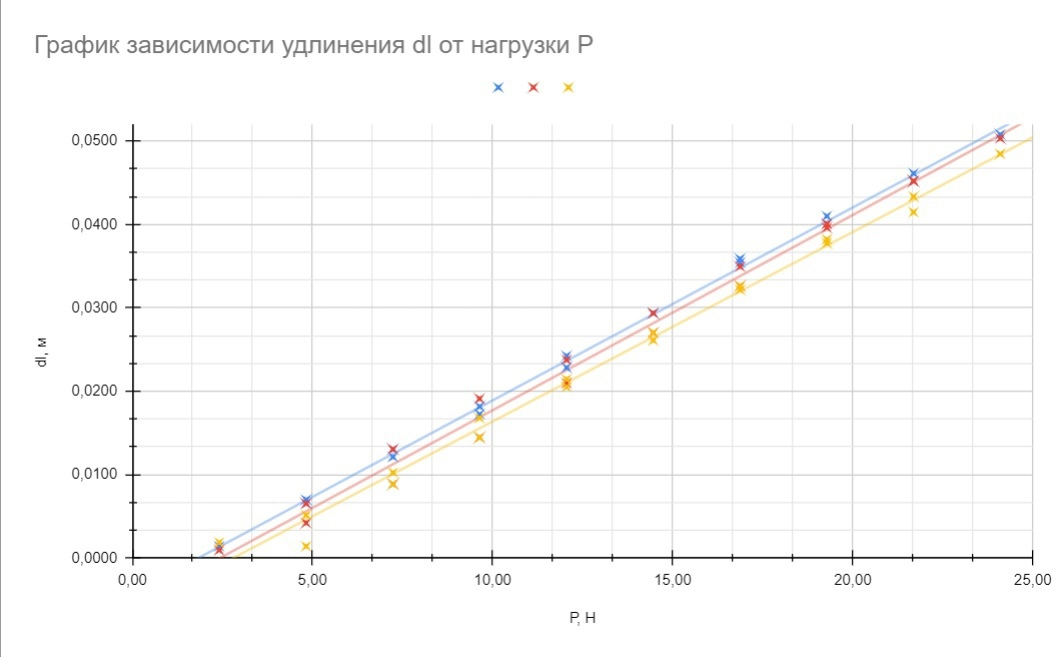
\includegraphics[width=14cm, height=9cm]{dlp.jpeg}
\end{center}
\begin{flushright}
{\scriptsize \textbf{Рис. 3.} \textbf {График зависисмости удлинения $dl$ от нагрузки $P$.}}
\end{flushright}
    
    Как видно по графику, зависимость линейна, однако прямая не проходит через начало координат, поскольку при малых нагрузках проволока распрямляется и начальные значения растяжения не учитываются.\\
    
    
    Угловой коэффициент полученной линейной зависимости - это величина, обратная к коэффициенту жесткости $k'$материала проволоки. Рассчитаем $k$ по методу наименьших квадратов:

    
\[k = \frac{<xy> - <y><x>}{<x^2> - <x>^2}\]    
    
    Погрешность определения значения $k$:
    
\[\sigma_{k} = k \sqrt{\frac{1}{N-1} \left(\frac{<y^2> - <y>^2}{<x^2> - <x>^2} - k^2\right)} = 0,00003\]
\[\varepsilon =  1,3 \%\]

\[\frac{1}{k} = k' = 432 713 \pm 5625 \frac{H}{m}\]


    По найденному значению коэффициента рассчитаем модуль Юнга для материала проволоки по формуле \eqref{модуль}.\\

    Погрешность определения Е:
    
\[\varepsilon_E = \sqrt{\varepsilon_k^2 + \varepsilon_l^2 + \varepsilon_s^2} = 1,4 \%\]

\[E = \frac{k' l}{S} = 182 \pm 3 G Pa\]

    
    
    
    
    
    
    
%---------------  
\section{Выводы}
  
    В данной работе мы нашли модуль Юнга исследуемого материала проволоки: $E = 182 \pm 3 $ ГПа. Основной вклад в погрешность определения модуля Юнга вносит погрешность нахождения жесткости материала проволоки $k'$, на которую влияют погрешности измерений расстояний длины проволоки и расстояния до шкалы, а также растяжения проволок из-за длительного воздействия грузов. Ближе всего по табличным значениям исследуемый материал к железу ($\approx 190 - 200$ ГПа). Можно предположить, что проволока изготовлена из сплава.\\
    
    Мы определили металл, из которого изготовлена исследуемая проволока при помощи прибора Лермантова по найденному модулю Юнга. Также найдена зависимость удлинения проволоки от действующей на нее силы. Мы убедились, что данная зависимость линейная и нашли по значениям экспериментально полученных данных коэффициент жесткости материала проволоки.
    


\end{document}

